\section{Results}
The results presented for each scenario include the energy produced, reactor 
deployment schedule, natural
uranium mass, \gls{HALEU} mass, and \gls{SWU} capacity as a function of time. 

\subsection{Scenario 1}
The amount of energy supplied by the \glspl{LWR} and the number of \glspl{LWR}
deployed as a function of time is shown in Figure \ref{fig:energy_rx_1}. 
\glspl{LWR} are first deployed in August of 1967, and the last 
\gls{LWR} is decommissioned in June of 2016. The maximum number of 
\glspl{LWR} deployed at one time is 109. The enery produced by the 
\glspl{LWR} follows with the number of reactors deployed. The maximum energy 
produced by the \glspl{LWR} is 102.46 GWe-y, and they produce 91.82 GWe-y 
in 2025.

\begin{figure}
    \centering 
    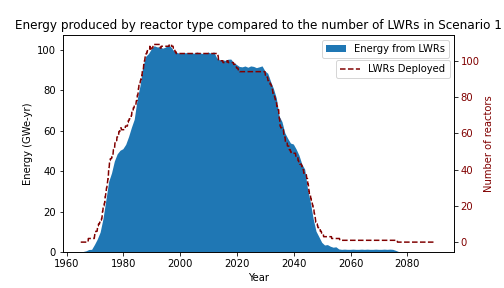
\includegraphics[scale=0.5]{figures/energy_scenario1.png}
    \caption{Energy supplied by \glspl{LWR} compared to the number of 
    \glspl{LWR} deployed in Scenario 1.}
    \label{fig:energy_rx_1}
\end{figure}

The next result is the mass of uranium sent to the \glspl{LWR} at each 
time step to fuel 
them, as shown in Figure \ref{fig:fuel_1}. Each of the \glspl{LWR} are 
defined to have an 18 month cycle length, with a third of the uranium 
mass replaced at each refueling outage. However, when a new reactor 
is deployed, it is deployed with an entire core of uranium which leads 
to the large increases in the mass of urnaium sent to the reactors, such 
as what is observed in 1983 and 2016. A maximum of 513.7 MT of uranium 
is required at one time for this scenario and an average of 96.2 MT/month 
of uranium is sent to the \glspl{LWR}. Prior to 2025, the average mass
of uranium sent to the \glspl{LWR} is 157.6 MT/month. 

\begin{figure}
    \centering 
    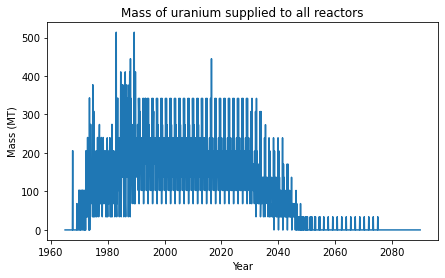
\includegraphics[scale=0.5]{figures/fuelsupply_scenarios_1.png}
    \caption{Mass of uranium sent to reactors in Scenario 1.}
    \label{fig:fuel_1}
\end{figure}

Finally, the \gls{SWU} capacity to produce fuel for the scenario, shown in 
Figure \ref{fig:swu_1}. The \gls{SWU} capacity required as a function of 
time follows the mass of uranium sent to the reactors, since the \gls{SWU}
is calculated based on those transactions. A maximum \gls{SWU} capacity of 
3950737.5 kg-\gls{SWU} and an average capacity of 740001.8 kg-\gls{SWU} is 
required for this scenario.

\begin{figure}
    \centering
    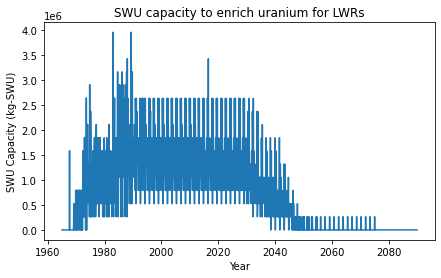
\includegraphics[scale=0.5]{figures/totalswu_scenarios_1.png}
    \caption{Total \gls{SWU} capacity required to produce fuel sent to the 
    reactors at each time step in Scenario 1.}
    \label{fig:swu_1}
\end{figure}

The deployment schedule of the \glspl{LWR} in this scenario is 
applied to each of the other scenarios, and therefore the material 
requirements of each of the following scenarios is the same as those 
of this scenario prior to 2025. 

\subsection{Scenario 2}
The energy produced by each type of reactor, the transition energy demand, 
and the deployment schedule of the \glspl{MMR} for Scenario 2 are shown in 
Figure \ref{fig:energy_rx_2}. Once the transition begins in 2025, there are 
clearly some time periods in which the energy demand of the scenario is 
not met. The first of these is between 2030-2050, with a maximum defecit 
of 5.7855 GWe-y in 2032. Other periods in which the energy demand is not met 
correspond to the decommissioning of \glspl{MMR} at the end of their lifetime 
and the deployment of new reactors, such as from 2062-2069. 

The first \glspl{MMR} are deployed starting in October 2031, and the 
maximum number of \glspl{MMR} deployed at one time in this scenario is 
9,182. The deployment of \glspl{MMR} in 2031 contributes to the inability to 
meet the energy demand of the scenario because the energy produced by 
\glspl{LWR} decreases to 89.35 GWe-y in 2030, before the \glspl{MMR} are 
deployed. Therefore, the reactors are deployed in a reactionary fashion to 
past energy production, as opposed to pre-emptively to forcasted energy 
production. 

\begin{figure}
    \centering 
    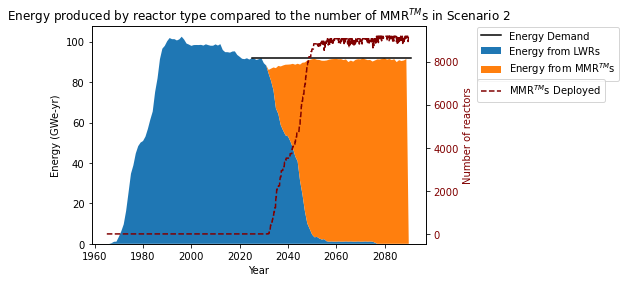
\includegraphics[scale=0.5]{figures/energy_scenario2.png}
    \caption{Energy supplied by each type of reactor compared to the number of 
    \glspl{MMR} deployed in Scenario 2.}
    \label{fig:energy_rx_2}
\end{figure}

Figure \ref{fig:totalfuel_2} shows the mass of uranium sent to all 
reactors in the scenario and Figure \ref{fig:haleu_2} shows the mass 
of uranium sent only to the \glspl{MMR} in the scenario. The \glspl{MMR} 
do not require refueling during their lifetime, so uranium is only 
sent to these reactors when they are initially deployed. This causes the 
large, sudden increases in uranium sent to these reactors and the periods of 
no uranium sent to them. A maximum of 719.25 MTU is sent to the \glspl{MMR} 
at one timestep and an average of 73.227 MTU/timestep is sent to the \glspl{MMR} 
once they are deployed in 2031.   

\begin{figure}
    \centering
    \begin{subfigure}{0.4\textwidth}
        \centering
        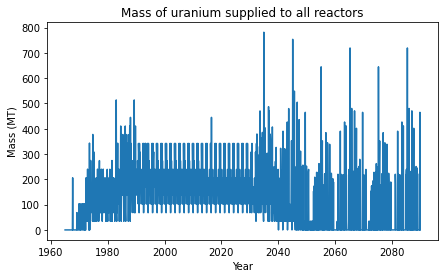
\includegraphics[scale=0.3]{figures/fuelsupply_scenarios_2.png}
        \caption{Total mass of uranium sent to all reactors at each time step.}
        \label{fig:totalfuel_2}
    \end{subfigure}
    \begin{subfigure}{0.4\textwidth}
        \centering
        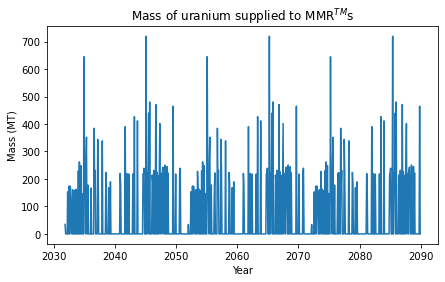
\includegraphics[scale=0.3]{figures/advancedRX_fuelsupply_scenarios_2.png}
        \caption{Total mass of uranium sent to \glspl{MMR} at each time step.}
        \label{fig:haleu_2}
    \end{subfigure}
    \caption{Uranium mass sent to reactors in Scenario 2.}
    \label{fig:fuel_2}
\end{figure}

Figure \ref{fig:swu_2} shows the \gls{SWU} capacity needed to 
enrich uranium for all reactors in the scenario to enrich uranium for 
just the \glspl{MMR}. There is a large difference in the \gls{SWU} 
capacity needed to enrich uranium for \glspl{LWR} and \glspl{MMR}. This 
is because the \gls{MMR} require a much larger mass of urnaium and 
urnaium at a higher enrchment level. A maximum of 20.3$\times 10^6$ kg-\gls{SWU}
is needed to enrich the uranium sent to \glspl{MMR} at any one time, and 
an average of 1.37$\times 10^6$ kg-\gls{SWU}/timestep is needed to enrich all of the 
uranium sent to the \glspl{MMR}. 


\begin{figure}
    \centering
    \begin{subfigure}{0.4\textwidth}
        \centering
        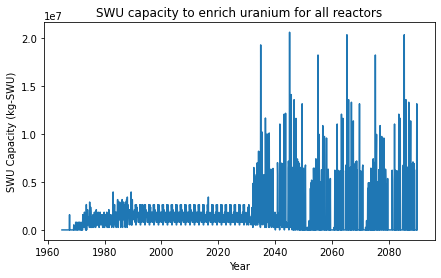
\includegraphics[scale=0.3]{figures/totalswu_scenarios_2.png}
        \caption{Total \gls{SWU} required to enrich uranium sent to all reactors at each time step.}
        \label{fig:totalswu_2}
    \end{subfigure}
    \begin{subfigure}{0.4\textwidth}
        \centering
        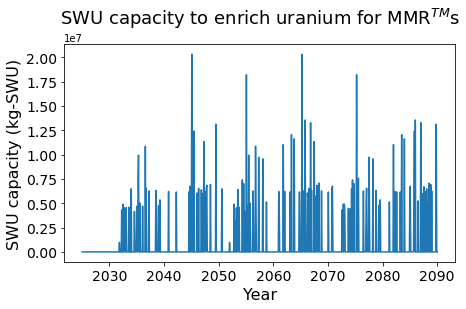
\includegraphics[scale=0.3]{figures/haleuSWU_scenarios_2.png}
        \caption{\gls{SWU} required to enrich uranium sent to \glspl{MMR} at each time step.}
        \label{fig:haleuswu_2}
    \end{subfigure}
    \caption{\gls{SWU} required to enrich natural uranium in Scenario 2.}
    \label{fig:swu_2}
\end{figure}

\subsection{Scenario 3}
Figure \ref{fig:energy_rx_3} shows the number of Xe-100 reactors deployed, 
the energy produced by each reactor type, and the energy demand of Scenario 3. 
There is the same gap between the energy produced and energy demand between 
2030-2050 that was observed in Scenario 2. However, there are no significant 
differences between the energy produced and energy demand of the scenario 
after 2050 because the Xe-100 reactors have a longer lifetime and there are 
no decreases in energy due to decommissioning of reactors. After 2050, the 
maximum difference between the energy produced and the demand is 0.057 GWe-y. 

Xe-100 reactors are deployed starting in October 2031, same as when \glspl{MMR}
are first deployed in Scenario 2. Combined with the consistency of the energy 
produced in Scenarios 2 and 3, this suggests that the \Cycamore ManagerInst 
deploys reactors on a reactionary basis instead of looking ahead to future 
requirements. A maximum of 1225 Xe-100 reactors are deployed in this scenario.

\begin{figure}
    \centering 
    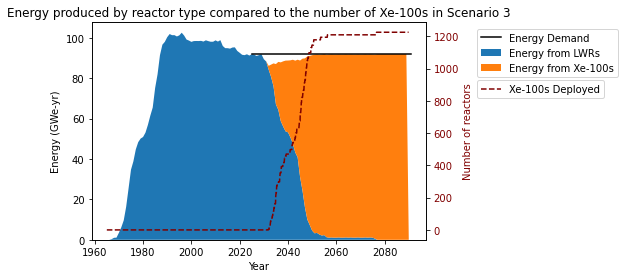
\includegraphics[scale=0.5]{figures/energy_scenario3.png}
    \caption{Energy supplied by each type of reactor compared to the number of 
    Xe-100s deployed in Scenario 3.}
    \label{fig:energy_rx_3}
\end{figure}

Figure \ref{fig:fuel_3} shows the mass of uranium sent to all reactors and 
just to the Xe-100 reactors in the simulation. The Xe-100 reactors 
require significantly less fuel than what is sent to the \glspl{LWR}, 
despite there being more \glspl{LWR} than Xe-100 reactors. Uranium 
is sent to the Xe-100 reactors every six months in the simulations, 
while it is sent to the \glspl{LWR} every 18 months. 

\begin{figure}
    \centering
    \begin{subfigure}{0.4\textwidth}
        \centering
        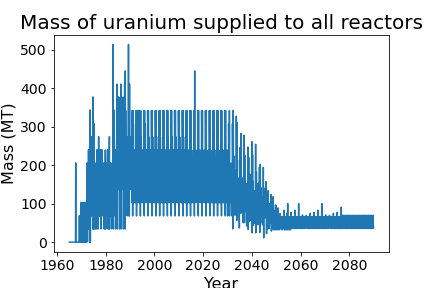
\includegraphics[scale=0.3]{figures/fuelsupply_scenarios_3.png}
        \caption{Total mass of uranium sent to all reactors at each time step.}
        \label{fig:totalfuel_3}
    \end{subfigure}
    \begin{subfigure}{0.4\textwidth}
        \centering
        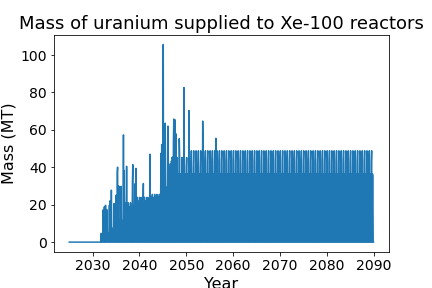
\includegraphics[scale=0.3]{figures/advancedRX_fuelsupply_scenarios_3.png}
        \caption{Total mass of uranium sent to Xe-100s at each time step.}
        \label{fig:haleu_3}
    \end{subfigure}
    \caption{Uranium mass sent to reactors in Scenario 3.}
    \label{fig:fuel_3}
\end{figure}

Figure \ref{fig:swu_3} shows the \gls{SWU} capacity needed to enrich 
uranium of all of the reactors in the scenario and for the uranium sent 
to just the Xe-100 reactors. There is no substantial change in the 
\gls{SWU} capacity needed to enrich uranium for \glspl{LWR} and for the Xe-100 
reactors. Enriching uranium for the Xe-100 reactors requires an average of 
8.23$\times 10^5$ kg-\gls{SWU}/timestep and a maximum of 3.64$\times 10^6$
kg-\gls{SWU}. 

\begin{figure}
    \centering
    \begin{subfigure}{0.4\textwidth}
        \centering
        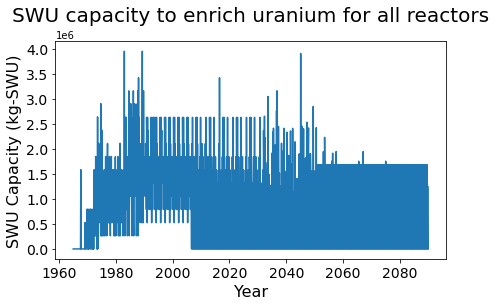
\includegraphics[scale=0.3]{figures/totalswu_scenarios_3.png}
        \caption{Total \gls{SWU} required to enrich uranium sent to all reactors at each time step.}
        \label{fig:totalswu_3}
    \end{subfigure}
    \begin{subfigure}{0.4\textwidth}
        \centering
        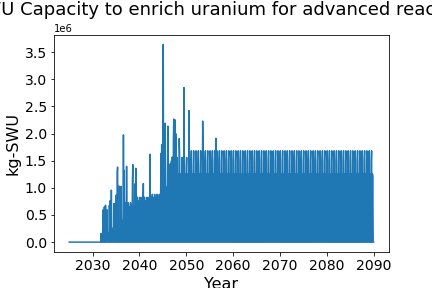
\includegraphics[scale=0.3]{figures/haleuSWU_scenarios_3.png}
        \caption{\gls{SWU} required to enrich uranium sent to Xe-100s at each time step.}
        \label{fig:haleuswu_3}
    \end{subfigure}
    \caption{\gls{SWU} required to enrich natural uranium in Scenario 3.}
    \label{fig:swu_3}
\end{figure}

\subsection{Scenario 4}

Figure \ref{fig:energy_rx_4} shows the number of \glspl{MMR} deployed, 
energy produced by each type of reactor, and the energy demand of the 
scenario. There is a small difference between the energy produced and the 
demand from 2026-2046, with a maximum difference of 4.51 GWe-y in 2032.
There are no other times in which the energy demand is not met by a 
significant amount, including when the \glspl{MMR} are decommissioned. 
After 2047 electricity is generally produced in surplus, up to 1.64 GWe-y, during 
this scenario. 

\glspl{MMR} are deployed starting in March 2029, and the maximum number 
of \glspl{MMR} deployed is 17656. 

\begin{figure}
    \centering 
    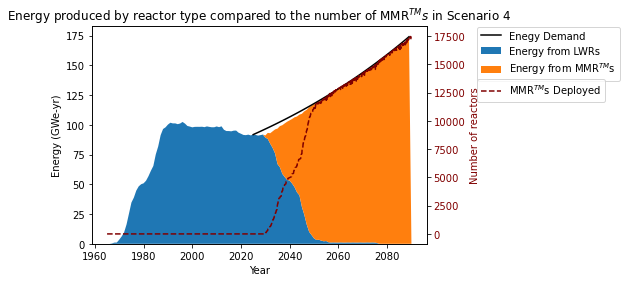
\includegraphics[scale=0.5]{figures/energy_scenario4.png}
    \caption{Energy supplied by each type of reactor compared to the number of 
    \glspl{MMR} deployed in Scenario 4.}
    \label{fig:energy_rx_4}
\end{figure}


\begin{figure}
    \centering
    \begin{subfigure}{0.4\textwidth}
        \centering
        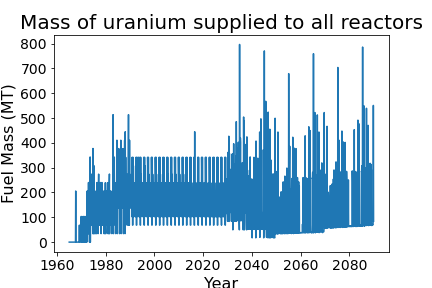
\includegraphics[scale=0.3]{figures/fuelsupply_scenarios_4.png}
        \caption{Total mass of uranium sent to all reactors at each time step.}
        \label{fig:totalfuel_4}
    \end{subfigure}
    \begin{subfigure}{0.4\textwidth}
        \centering
        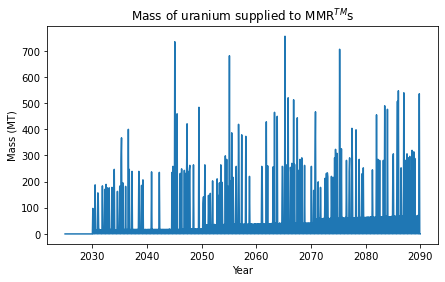
\includegraphics[scale=0.3]{figures/advancedRX_fuelsupply_scenarios_4.png}
        \caption{Total mass of uranium sent to \glspl{MMR} at each time step.}
        \label{fig:haleu_4}
    \end{subfigure}
    \caption{Uranium mass sent to reactors in Scenario 4.}
    \label{fig:fuel_4}
\end{figure}

Figure \ref{fig:swu_4} shows the \gls{SWU} capacity required to 
enrich uranium for all of the reactors in the scenario and the 
\gls{SWU} capacity to enrich uranium only for the \glspl{MMR} in 
the scenario. The \gls{SWU} capacity required to enrich uranium 
for the \glspl{MMR} is much higher than the capacity required to 
enrich uranium for the \glspl{LWR} in the scenario because
the \glspl{MMR} require a much higher mass of enriched uranium 
and a higher enrichment level. An average of 2.19$\times 10^6$ 
kg-\gls{SWU}/month is required to enrich uranium for the \glspl{MMR}
in this scenario, and a maximum of 2.15$\times 10^7$ kg-\gls{SWU}
is required to enrich the uranium that is sent to \glspl{MMR} at 
a single timestep. 

\begin{figure}
    \centering
    \begin{subfigure}{0.4\textwidth}
        \centering
        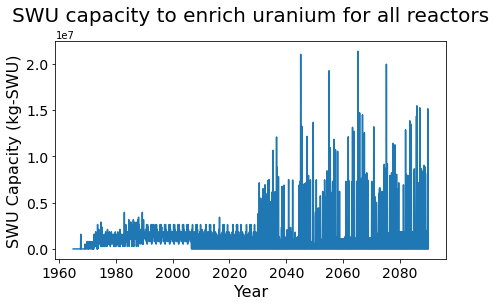
\includegraphics[scale=0.3]{figures/totalswu_scenarios_4.png}
        \caption{Total \gls{SWU} required to enrich uranium sent to all reactors at each time step.}
        \label{fig:totalswu_4}
    \end{subfigure}
    \begin{subfigure}{0.4\textwidth}
        \centering
        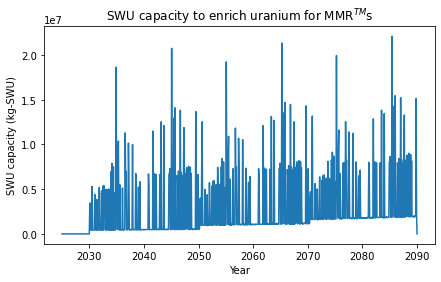
\includegraphics[scale=0.3]{figures/haleuSWU_scenarios_4.png}
        \caption{\gls{SWU} required to enrich uranium sent to \glspl{MMR} at each time step.}
        \label{fig:haleuswu_4}
    \end{subfigure}
    \caption{\gls{SWU} required to enrich natural uranium in Scenario 4.}
    \label{fig:swu_4}
\end{figure}


\subsection{Scenario 5}
Figure \ref{fig:energy_rx_5} shows the number of Xe-100 reactors, the 
energy produced by each type of reactor, and the energy demand of the 
scenario. There is a small gap in the energy produced and demand from 
2026-2046, the same as what was observed in Scenario 4. After this 
initial difference, there are no further significant differences between 
the energy produced and the demand. For most years after 2046 there 
is a surplus of energy, up to 1.64 GWe-y. 

The Xe-100 reactors are deployed starting in March 2029, same as when 
\glspl{MMR} are deployed in Scenario 4. The maximum number of Xe-100 
reactors deployed in the scenario is 2361. 

\begin{figure}
    \centering 
    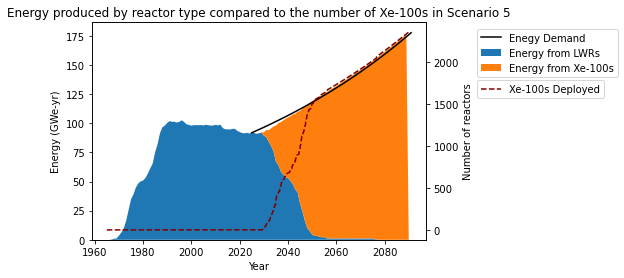
\includegraphics[scale=0.5]{figures/energy_scenario5.png}
    \caption{Energy supplied by each type of reactor compared to the number of 
    Xe-100s deployed in Scenario 5.}
    \label{fig:energy_rx_5}
\end{figure}

\begin{figure}
    \centering
    \begin{subfigure}{0.4\textwidth}
        \centering
        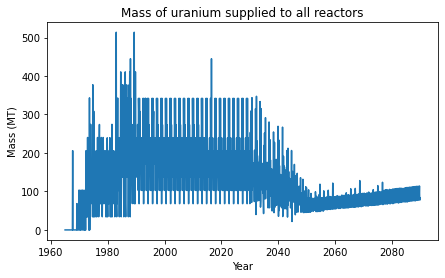
\includegraphics[scale=0.3]{figures/fuelsupply_scenarios_5.png}
        \caption{Total mass of uranium sent to all reactors at each time step.}
        \label{fig:totalfuel_5}
    \end{subfigure}
    \begin{subfigure}{0.4\textwidth}
        \centering
        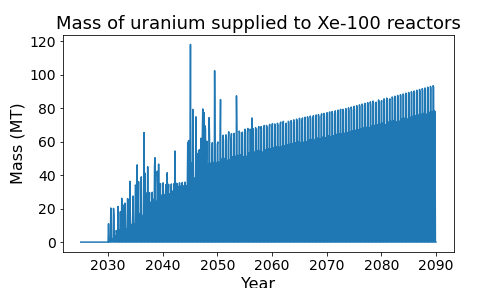
\includegraphics[scale=0.3]{figures/advancedRX_fuelsupply_scenarios_5.png}
        \caption{Total mass of uranium sent to Xe-100s at each time step.}
        \label{fig:haleu_5}
    \end{subfigure}
    \caption{Uranium mass sent to reactors in Scenario 5.}
    \label{fig:fuel_5}
\end{figure}

Finally, Figure \ref{fig:swu_5} shows the \gls{SWU} capacity required
to enrich the uranium sent to all of the reactors and just the Xe-100
reactors in the scenario at each time step. The \gls{SWU} capacity needed 
to enrich uranium for the Xe-100 reactors starts out at a similar 
amount to what is needed to enrich uranium for the \glspl{LWR}, but 
increases as the eenrgy demand and the number of reactors increases 
in the sceanrio. The \gls{SWU} capacity required to enrich uranium 
for the Xe-100 reactors becomes higher than the \gls{SWU} capacity 
required to enrich uranium for \glspl{LWR} despite the Xe-100 
reactors requiring a lower mass of uranium because of the higher 
enrichment level of the fuel. An average of 1.36$\times 10^6$ 
kg-\gls{SWU}/month is required 
to enrich uranium for the Xe-100 reactors, and a maximum of 
4.11$\times 10^6$ kg-\gls{SWU} is required to enrich the uranium sent to the 
Xe-100 reactors at one time step. 

\begin{figure}
    \centering
    \begin{subfigure}{0.4\textwidth}
        \centering
        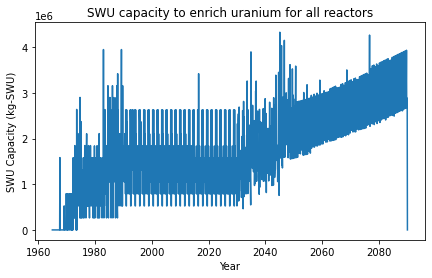
\includegraphics[scale=0.3]{figures/totalswu_scenarios_5.png}
        \caption{Total \gls{SWU} required to enrich uranium sent to all reactors at each time step.}
        \label{fig:totalswu_5}
    \end{subfigure}
    \begin{subfigure}{0.4\textwidth}
        \centering
        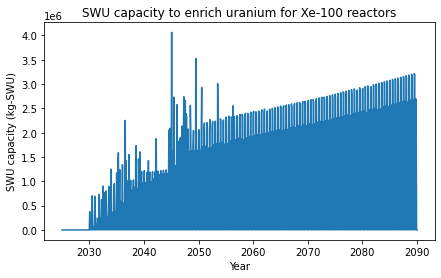
\includegraphics[scale=0.3]{figures/haleuSWU_scenarios_5.png}
        \caption{\gls{SWU} required to enrich uranium sent to Xe-100s at each time step.}
        \label{fig:haleuswu_5}
    \end{subfigure}
    \caption{\gls{SWU} required to enrich natural uranium in Scenario 5.}
    \label{fig:swu_5}
\end{figure}
